Improvement of Scalar Multiplication by Skew Frobenius Map with Multi-Scalar Multiplication for KSS Curve

Scalar multiplication over higher degree rational point groups is often regarded as the bottleneck for faster pairing based cryptography.
This paper has presented a skew Frobenius mapping technique in the sub-field isomorphic \textit{sextic twisted} curve of  Kachisa-Schaefer-Scott (KSS)  pairing friendly curve of \textit{embedding degree} 18  in the context of Ate based pairing. 
Utilizing the skew Frobenius map along with multi-scalar multiplication procedure, an efficient scalar multiplication method for KSS curve is proposed in the paper.
In addition to the theoretic proposal, this paper has also presented a comparative simulation of the proposed approach with plain binary method, sliding window method and non-adjacent form (NAF) for scalar multiplication. The simulation shows that the proposed method is about 60 times faster than plain implementation of other compared methods.
\section{Introduction}

Pairing based cryptography has attracted many researchers since Sakai et al. \cite{sakai} and Joux et al. \cite{joux} independently proposed a cryptosystem based on elliptic curve pairing. This has encouraged to invent several innovative pairing based cryptographic applications such as broadcast encryption \cite{boradcast} and group signature authentication \cite{group_sign_1}, that has increased the popularity of pairing based cryptographic research.
But using pairing based cryptosytem in industrial state is still restricted by its expensive operational cost with respect to time and computational resources in practical case. 
In order to make it practical, several pairing techniques such as Ate \cite{ate}, Optimal-ate \cite{op_ate_p}, twisted Ate \cite{twisted_ate}, $\chi$-Ate \cite{chibasedBN} and \textit{sub-field twisted} Ate \cite{devegili} pairings have gained much attention since they have achieved quite efficient pairing calculation in certain pairing friendly curve. 
Researchers still continues on finding efficient way to implement pairing to make it practical enough for industrial standardization. 
In such consequences, this paper focuses on a peripheral technique of Ate-based pairings  that is scalar multiplication defined over Kachisa-Schaefer-Scott (KSS) curve \cite{kss} of embedding degree 18. 

In general, pairing is a bilinear map of two rational point groups $\g1$ and $\g2$ to a multiplicative group $\g3$ \cite{Silverman}.
The typical notation of pairing is $\g1 \times \g2 \rightarrow \g3$.
In  Ate-based pairing, $\g1$, $\g2$ and $\g3$ are defined as:
\begin{eqnarray}\label{eq:g_1}
\g1 & = &  E(\F{p}{k}) [r] \cap \text{Ker}(\pi_p - [1]), \nonumber \\
\g2 & = &  E(\F{p}{k}) [r] \cap \text{Ker}(\pi_p - [p]), \nonumber \\
\g3 & = & \mF{p}{k}/(\mF{p}{k})^r, \nonumber
\end{eqnarray}
\begin{equation}
\alpha : \g1 \times \g2 \rightarrow \g3,  \nonumber
\end{equation}
where $\alpha$ denotes Ate pairing.
Pairings are often defined over certain extension field $\FQK$, where $p$ is the prime number, also know as characteristics  and $k$  is the minimum extension degree for pairing also called \textit{embedding} degree. 
The set of rational points $E(\FQK)$ are defined over a certain pairing friendly curve of embedded extension field of degree $k$.
This paper has considered Kachisa-Schaefer-Scott (KSS) \cite{kss} pairing friendly curves of emebdding degree $k=18$ described in \cite{taxonomy}.

Scalar multiplication is often considered to be  one of the most time consuming operation in cryptographic scene. 
Efficient scalar multiplication is one of the important factors for making the pairing practical over KSS curve.
%  depends on several factors such as efficient pairing algorithm, efficient extension field arithmetic and . 
There are several works \cite{nogami}\cite{sakemi_skew} on efficiently computing scalar multiplication defined over Barreto-Naehrig\cite{BN} curve along with efficient extension field arithmetic \cite{ef_ex}. 
This paper focuses on efficiently performing scalar multiplication on rational points defined over rational point group $\g2$ by scalar $s$, since scalar multiplication is required repeatedly in cryptographic calculation.
However in asymmetric pairing such as Ate-based pairing, scalar multiplication of $\g2$ rational points is important as no mapping function is explicitly given between $\g1$ to $\g2$.
By the way, as shown in the definition, $\g1$ is a set of rational points defined over prime field and there are several researches \cite{sakemi_skew} for efficient scalar multiplication in $\g1$.
The common approach to accelerate scalar multiplication are log-step algorithm such as binary and non-adjacent form (NAF) methods, but more efficient approach is to use Frobenius mapping in the case of $\g2$ that is defined over $\F{p}{k}$.
Moreover when sextic twist of the pairing friendly curve exists, then we apply skew Frobenius map on the isomorphic sextic-twisted sub-field rational points. Such technique will reduce the computational cost in a great extent.
In this paper we have exploited the sextic twisted property of KSS curve and utilized skew Frobenius map to reduce the computational time of scalar multiplication on $\g2$ rational point. 
Utilizing the relation $z \equiv -3p + p^4 \bmod {r}$,\footnote{$z$ is the mother parameter of KSS curve and $z$ is about six times smaller than the size of order $r$.} derived by Aranha et al,\cite{aranha} and the properties of $\g2$ rational point, the scalar can be expressed as $z$-adic representation.
Together with skew Frobenius mapping and $z$-adic representation the scalar multiplication can be further accelerated.  
We have utilized this relation to construct $z$-adic representation of scalar $s$ which is introduced in section 3. 
In addition with Frobenius mapping and $z$-adic representation of $s$, we applied the multi-scalar multiplication technique to compute elliptic curve addition in parallel in the proposed scalar multiplication.
We have compared our proposed method with three other well studied methods named binary method, sliding-window method and non-adjacent form method. 
The comparison shows that our proposed method is about 60 times faster than the plain implementations of above mentioned methods in execution time. The comparison also reveals that the proposed method requires more than 5 times less elliptic curve doubling than any of the compared methods.

The rest of the paper is organized as follows. 
The fundamentals of elliptic curve arithmetic, scalar multiplication along with KSS curve over $\FQEN$ extension field and \textit{sextic twist} of KSS curve are described in section 2.
In section 3, this paper describes the proposal in details. The experimental result is presented in section 4 which shows that our scalar multiplication technique on $\g2$ rational points of KSS curve can be accelerated by 60 times than plain implementation of binary, sliding-window and NAF methods. Finally section 5 draws the conclusion with some outline how this work can be enhanced more as a future work.

Throughout this paper, $p$ and $k$ denote characteristic and embedding extension degree, respectively. $\FQK$ denotes $k$-th extension field over prime field $\Fp$ and $\mF{p}{k}$ denotes the multiplicative group in $\FQK$ .

The process of getting $z$-adic representation and using it for scalar multiplication over KSS curve is presented in 17th World Conference on Information Security Applications (WISA 2016), Jeju, Korea. It will be published in the conference proceedings from Springer LNCS.  For the convenience of describing the total procedure, here we will discus $z$-adic representation in section 3.

\section{Preliminaries}
In this section we will go through the fundamental background of elliptic curves and its operations. We will briefly review elliptic curve scalar multiplication. After that pairing friendly curve of embedding degree $k=18$, i.e., KSS curve and its properties will be introduced briefly.
\subsection{Elliptic curve}
An elliptic curve \cite{ecc_book} defined over $\Fp$ is generally represented by \textit{affine coordinates} \cite{Silverman} as follows;
%Let $\Fp$ be a prime field. Elliptic curve over $\Fp$ is defined as,
\begin{equation}\label{ec_curve}
E/\Fp : y^2=x^3+ax+b,
\end{equation}
where $ 4a^3+27b^2 \neq 0$ and $a,b \in \Fp$. A pair of coordinates $x$ and $y$ that satisfy \eqref{ec_curve} are known as \textit{rational points} on the curve. 
%Points satisfying \eqref{ec_curve} are known as rational points on the curve.
% Now let us denote the base extension field as $\Fq$. 
%The set of rational points over $\Fp$, including point at infinity $\mathcal{O}$ is denoted by $\EFP$. 

\subsubsection{Point addition.}
Let $E(\f{p})$ be the set of all rational points on the curve $E$ including the point at infinity $\mathcal{O}$.
$\SEFP$ denotes the order of $\EFP$.
Let us consider two rational points using affine coordinates as $P_1= (x_1, y_1)$, $P_2 = (x_2, y_2)$, and their addition $R = P_1 + P_2$, where $\textit{R} = (x_3, y_3)$ and $P_1, P_2, R \in E(\Fp)$. Then the $x$ and $y$ coordinates of $R$ are calculated as follows:

\begin{subequations}
\begin{eqnarray}\label{eq:point_add}
x_3 & = & \lambda^2-x_1-x_2 ,\\
 y_3 & = &(x_1-x_3)\lambda - y_1, 
\end{eqnarray}
where \mbox{$\lambda$} is given as follows:
\begin{equation}\label{eq:point_solpe}
\textstyle \lambda = 
\begin{cases}
 \textstyle \frac{y_2 - y_1}{ x_2 -x_1}; \quad \mbox{$P_1 \neq P_2$},\\
 \textstyle \frac{3x_1^2+a}{2y_1}; \quad  \mbox{$P_1 = P_2$},\\
\end{cases}
\end{equation}
\end{subequations}
$\lambda$ is the tangent at the point on the curve and $\cal O$ is the additive unity in $E(\f{p})$. If $P_1 \neq P_2$ then $P_1+P_2$ is called elliptic curve addition (ECA). If $P_1=P_2$ then $P_1+P_2=2P_1$, which is known as elliptic curve doubling (ECD). 

\subsubsection{Scalar multiplication}
Let scalar $s$ is $0 \leq s < r$, where $r$ is the order of the target rational point group. Scalar multiplication of rational points $P_1$, denoted as $[s]P_1$ is calculated by $(s-1)$-times additions of $P_1$ as,
\begin{equation}\label{scalar_mul}
[s]P_1 = \sum_{i=0}^{s-1} P_1, \quad \text{$0 \leq s < r$},
\end{equation}
When $s = r$, then $[r]P_1 = \mathcal{O}$ where $r$ is the order of the curve. Let $[s]P_1 = P_2$, and value of $s$ is not obtained, then the solving $s$ from $P_1$ and $P_2$ is known as elliptic curve discrete logarithm problem (ECDLP). The difficulty level of solving ECDLP defines the security strength of elliptic curve cryptography.

\subsection{KSS curve}
In  \cite{kss}, Kachisa, Schaefer, and Scott proposed a family of non super-singular Brezing-Weng pairing friendly elliptic curves using elements in the cyclotomic field. In what follows this paper considers the KSS curve of  embedding degree $k=18$ since it holds \textit{sextic twist}. 
The equation of KSS curve defined over $\FQEN$ is given as follows:
\begin{equation}\label{eq:KSS_curve}
E:Y^2=X^3+b, \quad \mbox{($b \in \Fp$)},
\end{equation}
where $b \neq 0$ and $X,Y \in \FQEN$. Its characteristic $p$, Frobenius trace $t$ and order $r$ are given systematically by using an integer variable $z$ as follows:
\begin{subequations}
\begin{eqnarray}
p(z) &= & (z^8 +5z^7 +7z^6 +37z^5 +188z^4 +259z^3  \nonumber \\ 								
& & + 343z^2 +1763z+2401)/21,\\\label{eq:kss_char}
r(z) &= &(z^6 + 37z^3 + 343)/343,\label{eq:kss_degree}  \\
t(z) &=& (z^4 + 16z + 7)/7, \label{eq:kss_trace} 
\end{eqnarray}
\end{subequations} 
where $z$ is such that $z \equiv 14$ (mod $42$) and the $\rho$ value is $\rho = (\log_2 p/\log_2 r) \approx 1.33$.

In some previous work of  Aranha et al. \cite{aranha} and Scott et al. \cite{kss_param} has mentioned that the size of the characteristics $p$ to be 508 to 511-bit with order $r$ of 384-bit  for 192-bit security level.  
Therefore this paper used parameter settings according to the suggestion of \cite{aranha} for 192 bit security on KSS curve in the simulation implementation. In the recent work, Kim et al. \cite{kim_ecdlp} has suggested to update the key sizes in pairing-based cryptography due to the  development of new discrete logarithm problem over finite field. The parameter settings used in this paper doesn't completely end up at the 192 bit security level according to \cite{kim_ecdlp}. However the parameter settings used in this paper in order to show the resemblance of the proposal with the experimental result.

\subsection{$\FQEN$ extension field arithmetic}
Pairing based cryptography requires to perform arithmetic operation in extension fields of degree $k \geq 6$\cite{Silverman}. In the previous works of Bailey et al. \cite{OEF} explained optimal extension field by towering by using irreducible binomials.  In this paper extension field  $\FQEN$ is represented as a tower of sub field to improve arithmetic operations. 

Let $(p-1)$ is divisible by 3 and $c$ is a quadratic and cubic non residue in $\Fp$. In KSS curve \cite{kss}, where $k=18$, $\FQEN$ is constructed  with irreducible binomials by the following towering scheme.
\begin{equation}
\begin{cases}
\F{p}{3} = \F{p}{}[i]/(i^3-c),  \text{where $c = 2$ is the best choice,}\nonumber \\ 
\F{p}{6} = \F{p}{3}[v]/(v^2-i), \nonumber \\ 
\F{p}{18} = \F{p}{6}[\theta]/(\theta^3-v). \nonumber \\ 
\end{cases}
\end{equation}\label{KSS_towering}
where the base extension field is $\FQTH$ for the \textit{sextic twist} of KSS curve.

\subsubsection{Frobenius mapping of rational point in  $E(\FQEN)$.}
Let $(x,y)$ be certain rational point in $E(\FQEN)$. 
Frobenius map $\pi_p : (x,y) \mapsto  (x^p,y^p)$ is the $p$-th power of the rational point defined over $\FQEN$. 
Sakemi et al. \cite{sakemi_skew} showed an efficient scalar multiplication by applying skew Frobenius mapping in the context of Ate-based pairing in BN curve of embedding degree $k=12$.  In this paper we have utilized skew Frobenius mapping technique for efficient scalar multiplication for the KSS curve.

\subsection{Sextic twist of KSS curve}
Let the embedding degree $k = 6e$, where $e$ is positive integer, \textit{sextic} twist is given as follows:
\begin{eqnarray}
E:  \quad y^2 & = & x^3+b, \quad b \in \Fp, \\
E'_6: \quad y^2 & =  & x^3+bu^{-1},
\end{eqnarray}  
where $u$ is a quadratic and cubic non residue in $E(\F{p}{e})$ and $3|(p^e-1)$.  Isomorphism between $E'_6(\F{p}{e})$ and $E(\F{p}{6e})$, is given as follows:
\begin{eqnarray}
\psi_6 : \begin{cases}
E'_6(\F{p}{e}) \rightarrow E(\F{p}{6e}),\\
(x,y) \quad \mapsto (xu^{1/2},yu^{1/2}).
\end{cases}
\end{eqnarray}
In context of Ate-based pairing for KSS curve of embedding degree 18, sextic twist is considered to be the most efficient.

\section{Improved Scalar Multiplication for $\g2$ rational point}
This section will introduce the proposal for efficient scalar multiplication of $\g2$ rational points defined over KSS curve of embedding degree $k=18$ in context of Ate-based pairing. 
An overview the proposed method is given next before diving into the detailed procedure.
\subsubsection{Overview of the proposal} 
Figure \ref{process} shows an overview of overall process of proposed scalar multiplication.
\begin{figure*}[ht]
\centering
%\resizebox{0.7\columnwidth}{!}{
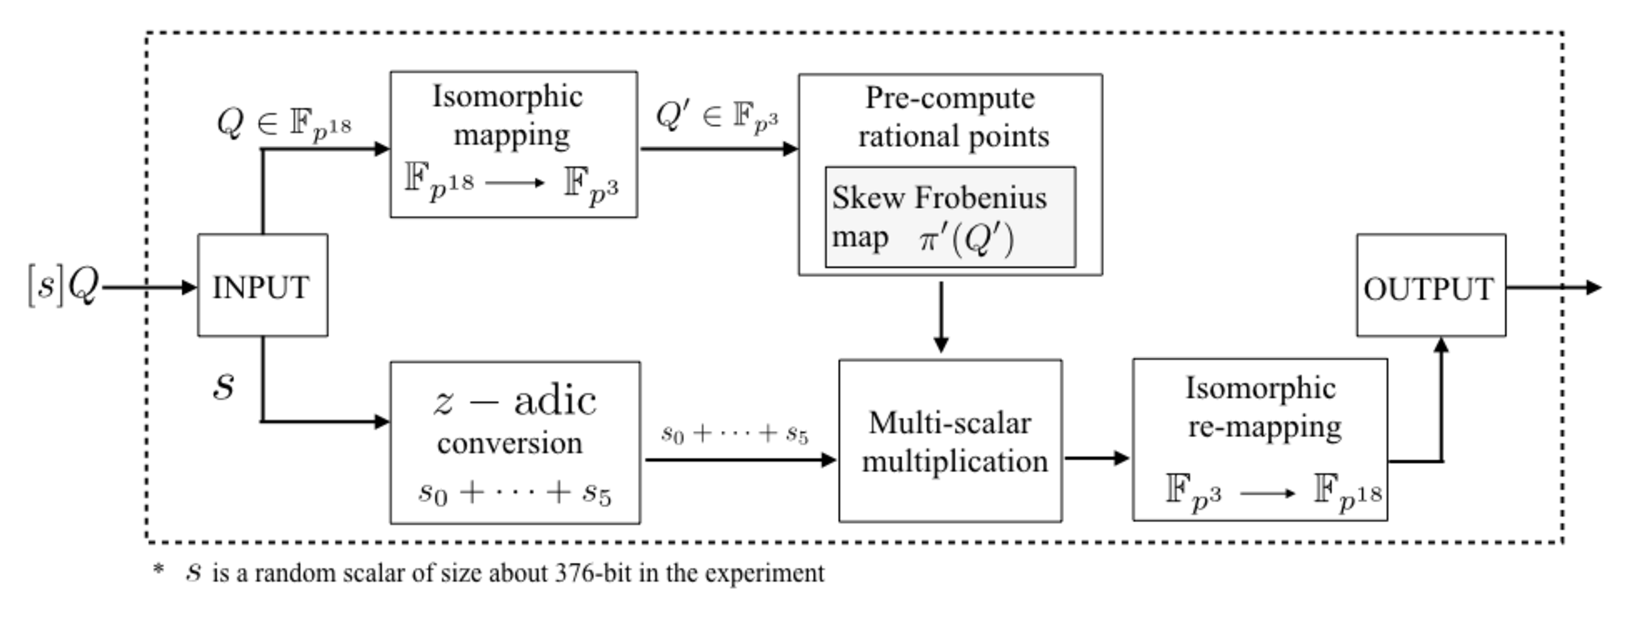
\includegraphics[width=6.5in]{process.eps}
\caption{Overview of the proposed scalar multiplication.}
\label{process}
\end{figure*}
Rational point groups $\g1$, $\g2$ and multiplicative group $\g3$ groups will be defined at the beginning. Then a rational point $Q\in \g2 \subset E(\F{p}{18})$ will be calculated.
$Q$ has a  special vector representation with 18 $\Fp$ elements for each coordinates. 
A random scalar $s$ will be considered for scalar multiplication of $[s]Q$ which is denoted as input in  Figure \ref{process}. After that we will consider an isomorphic map of rational point $Q\in \g2 \subset E(\F{p}{18})$ to its sextic twisted rational point $Q' \in \g2' \subset E'(\F{p}{3})$. At the same time we will obtain the $z$-adic  representation of the scalar $s$. Next the some rational points defined over $E'(\FQTH)$ will be pre-computed by applying the skew Frobenius mapping. After that a multi-scalar multiplication technique will be applied to calculate the scalar multiplication in parallel. The result of this scalar multiplication will be defined over $\FQTH$. Finally the result of the multi-scalar multiplication will be re-mapped to rational point in $E(\FQEN)$ to get the final result.

\subsection{\g1, \g2 and \g3 groups} In the context of pairing-based cryptography, especially on KSS curve, three groups $\g1, \g2$, and $\mathbb{G}_3$ are considered. From \cite{mori}, we define $\g1$, $\g2$ and $\g3$ as follows:
\begin{eqnarray}\label{eq:g1}
\g1 & = &  E(\F{p}{18}) [r] \cap \text{Ker}(\pi_p - [1]), \nonumber \\
\g2 & = &  E(\F{p}{18}) [r] \cap \text{Ker}(\pi_p - [p]), \nonumber \\
\g3 & = & \mF{p}{18}/(\mF{p}{18})^r, \nonumber
\end{eqnarray}
\begin{equation}
\alpha : \g1 \times \g2 \rightarrow \g3,
\end{equation}
where $\alpha$ denotes Ate pairing. In the case of KSS curve, $\g1, \g2$ are rational point groups and $\mathbb{G}_3$ is the multiplicative group in $\FQEN$. They have the same order $r$. 

In context of KSS curve, let us consider a rational point $Q\in \g2 \subset E(\F{p}{18})$ where $Q$ satisfies the following relations,
\begin{eqnarray}\label{eq:Q_rel1}
\big[p+1-t\big]Q & = & \cal O, \nonumber \\
\big[t-1\big]Q  & = & \big[p\big]Q.
\end{eqnarray}
\begin{eqnarray}\label{eq:Q_rel2}
[\pi_p -p]Q & = &\cal O, \nonumber \\
\pi_p(Q) & = & [p]Q.
\end{eqnarray}
where  $[t-1]Q = \pi_p(Q)$, by substituting $[p]Q$ in \eqref{eq:Q_rel1}.


\subsection{Isomorphic mapping between $Q$ and $Q'$}
Let us consider $E$ is the KSS curve in base field $\FQTH$  and $E'$ is sextic twist of $E$ given as follows: 
\begin{eqnarray}
E:y^2 & = &x^3+b,\\
E':y^2 & = & x^3+bi, \label{eq:KSS_Twist}
\end{eqnarray}
where $b \in \Fp$; $x, y, i \in \FQTH$ and basis element $i$ is the quadratic and cubic non residue in $\FQTH$.

Rational point $Q\in \g2 \subset E(\F{p}{18})$ has a  special vector representation with 18 $\Fp$ elements for each $x_Q$ and $y_Q$ coordinates.
Figure \ref{fig:Q_structure} shows the structure of the coefficients of $Q \in \FQEN$ and its sextic twisted isomorphic rational point $Q' \in \FQTH$ in KSS curve.
\begin{figure}[!htb]
\centering
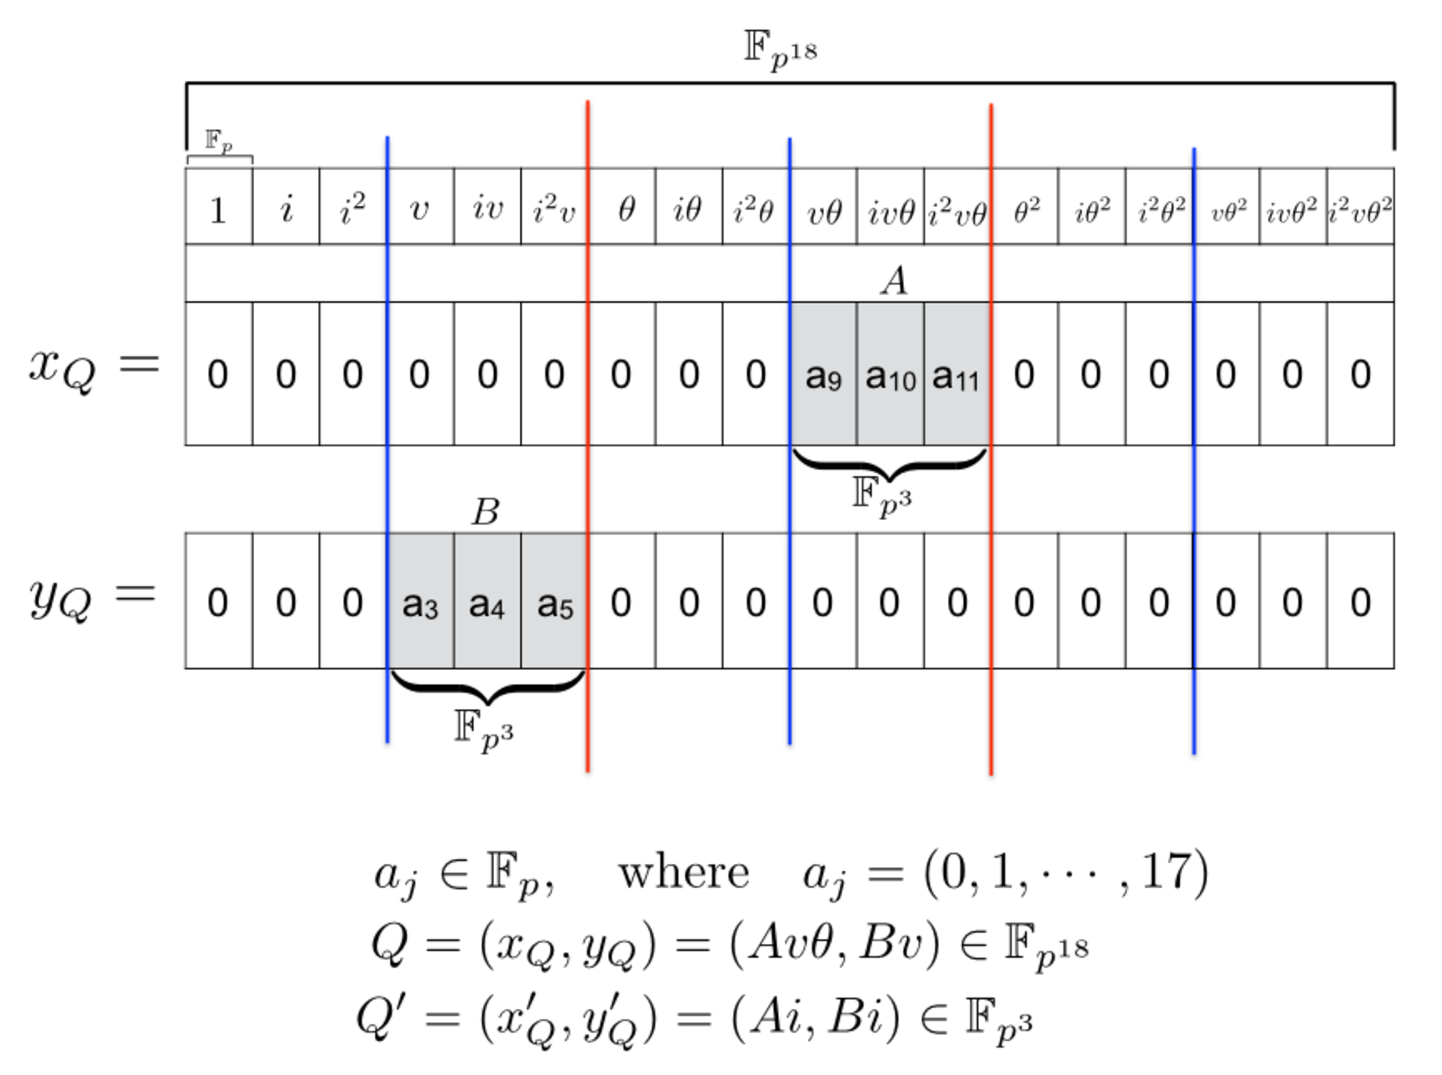
\includegraphics[width=1.0\columnwidth]{structure.eps}
\caption{ $Q \in \FQEN$ and its sextic twisted isomorphic rational point $Q' \in \FQTH$ structure in KSS curve.}
\label{fig:Q_structure}
\end{figure}
Among 18 elements, there are 3 continuous nonzero $\Fp$ elements which belongs to a $\FQTH$ element. The other coefficients are zero.
In this paper, considering parameter settings given in Table \ref{parameters} of section 4; $Q$ is given as $Q = (Av\theta, Bv)$,  showed in Figure \ref{fig:Q_structure}, where $A, B \in \FQTH$ and $v$ and $\theta$ are the basis elements of $\F{p}{6}$ and $\FQEN$ respectively. 

Let us consider the sextic twisted isomorphic sub-field rational point of $Q$ as $Q' \in \g2' \subset E'(\F{p}{3})$ and $x'$ and $y'$ as the coordinates of $Q'$.

\subsubsection{Mapping $Q = (Av\theta, Bv)$  to the rational point  $Q' = (x',y')$}

Let's multiply  $\theta^{-6}$ with both side of \eqref{eq:KSS_Twist}, where $i=\theta^6$ and $v = \theta^3$.
\begin{equation}\label{eq.sextic_div_theta}
E':  \Big(\frac{y}{\theta^3}\Big)^2  = \Big(\frac{x}{\theta^2}\Big)^3+ b.
\end{equation}
 Now $\theta^{-2}$ and $\theta^{-3}$ of  \eqref{eq.sextic_div_theta} can be represented as follows:
 \begin{subequations}
 \begin{eqnarray}
 \theta^{-2} &  = & i^{-1}\theta^{4}, \label{thta2_4} \\
 \theta^{-3} &  = & i^{-1}\theta^{3}.\label{thta_3} 
 \end{eqnarray}
 \end{subequations}
Let us represent $Q = (Av\theta, Bv)$  as follows:
\begin{equation}\label{18_to3}
Q  =  (A\theta^4, B\theta^3), \quad \text{where $v=\theta^3$}.
\end{equation}
From \eqref{thta2_4} and \eqref{thta_3} $ \theta^4 = i\theta^{-2}$ and $\theta^3 = i\theta^{-3}$  is substituted in \eqref{18_to3}  as 
follows:
\begin{equation}\label{18_to3.1}
Q  =  (Ai\theta^{-2}, Bi\theta^{-3}),
\end{equation}
where $Ai = x'$ and $Bi = y'$ are the coordinates of $Q' =(x',y') \in \FQTH$. 
 From the structure of $\FQEN$, given in \ref{KSS_towering}, this mapping has required no expensive arithmetic operation. Multiplication by the basis element $i$ in $\FQTH$ can be done by 1 bit wise left shifting since $c=2$ is considered for towering in \ref{KSS_towering}.


\subsection{$z$-adic representation of scalar $s$} 
In context of KSS curve, properties of $Q$ will be obtained to define the \eqref{eq:Q_rel2} relation.
Next, a random scalar $s$ will be considered for scalar multiplication of $[s]Q$. Then $(t-1)$-adic representation of $s$ will be considered as Figure \ref{fig:t_adic}. Here $s$ will be divided into two smaller coefficients $S_H$, $S_L$ where  $S_L$ denotes lower bits of $s$,  will be nearly equal to the size of $(t-1)$. On the other hand the higher order bits $S_H$ will be the half of the size of $(t-1)$. Next, $z$-adic representation of $S_H$ and $S_L$ will be considered. Figure \ref{fig:z_adicl}, shows the $z$-adic representation from where we find that scalar $s$ is divided into 6 coefficients of $z$, where the size of $z$ is about $1/4$ of that of $(t-1)$ according to \eqref{eq:kss_trace}. 

Figure \ref{fig:t_adic} shows $(t-1)$-adic representation of scalar $s$. 
\begin{figure}[!ht]
\centering
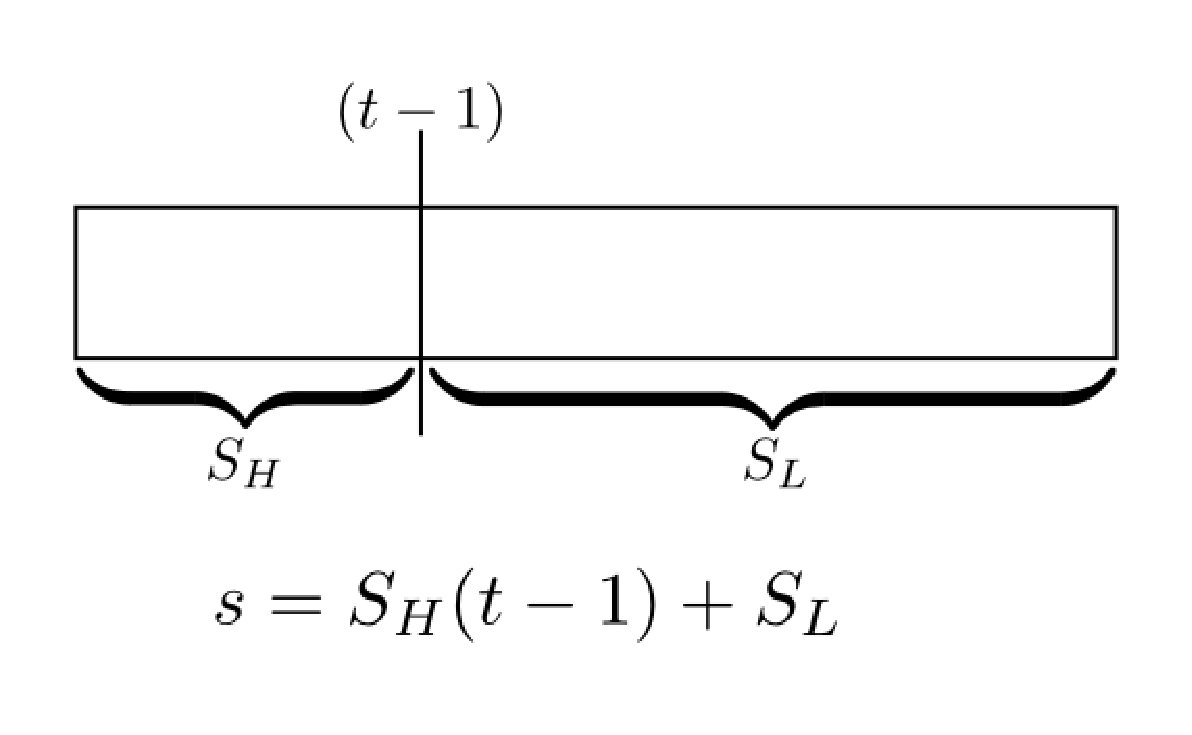
\includegraphics[width=0.7\columnwidth]{t_adic.eps}
\caption{$(t-1)$ -adic representation of scalar $s$.}
\label{fig:t_adic}
\end{figure}

Figure \ref{fig:z_adicl} shows the  $z$-adic representation of scalar $s$. 
\begin{figure}[!ht]
\centering
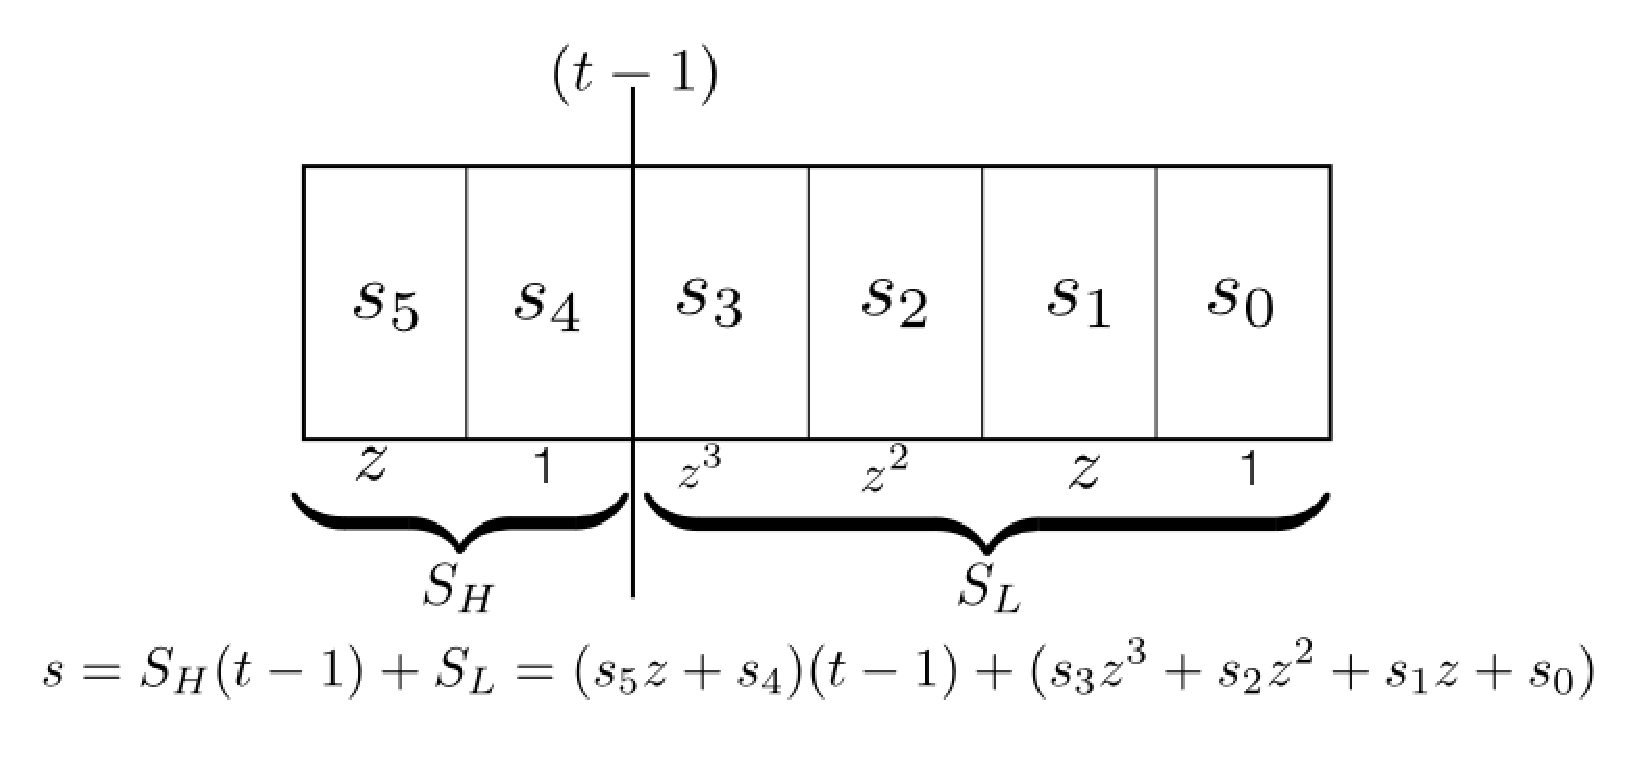
\includegraphics[width=1.0\columnwidth]{z_adic.eps}
\caption{$z$-adic and $(t-1)$-adic representation of scalar $s$.}
\label{fig:z_adicl}
\end{figure}
In the previous work on optimal-ate pairing, Aranha et al. \cite{aranha} derived a relation from the parameter setting of KSS curve as follows:
\begin{equation}\label{eq:aranha_relation}
z+3p-p^4 \equiv 0 \bmod {r},
\end{equation}
where $z$ is the \textit{mother parameter} of KSS curve which is about six times smaller than order $r$. 

Since $Q$ is mapped to its ismorphic sextic twisted rational point $Q'$, therefore we can consider scalar multiplication $[s]Q'$ where $0 \leq s < r$. $[s]Q'$ will be calculated in $\FQTH$ and eventually the result will be mapped to $\FQEN$ to get the final result. From \eqref{eq:kss_degree} we know $r$ is the order of KSS curve  where $[r]Q=\cal O$. Here, the bit size of $s$ is nearly equal to $r$. In KSS curve $t$ is  $4/6$ times of  $r$. Therefore, let us first consider $(t-1)$-adic representation of $s$ as follows:
\begin{equation}\label{eq:t-1_adic}
s =  S_H(t-1)+S_L,
\end{equation}
where $s$ will be separated into two coefficients $S_H$ and $S_L$. $S_L$ will be nearly equal to the size of $(t-1)$ and $S_H$ will be about half of $(t-1)$. 
In what follows, $z$-adic representation of $S_H$ and $S_L$ is given as:
\begin{eqnarray}\label{eq:scalar_mul_Q}
S_H & =  & s_5+ s_4,\nonumber \\
S_L & = & s_3 z^3+s_2 z^2+s_1 z+s_0.\nonumber 
\end{eqnarray}
Finally $s$ can be represented as 6 coefficients as follows:
\begin{eqnarray}\label{eq:sclar_final_rep}
s & =  & \sum_{i=0}^{3} s_iz^i + (s_4+s_5z)(t-1),\nonumber \\
s & = & (s_0+s_1z) + (s_2 +s_3z)z^2 +(s_4+s_5z)(t-1).
\end{eqnarray}

\subsubsection{Reducing number of  Elliptic Curve Doubling (ECD) in $[s]Q'$.}
Let us consider a scalar multiplication of $Q' \in \g2'$ in \eqref{eq:sclar_final_rep} as follows:
\begin{equation}\label{eq:proposed_scm_1}
[s]Q' =  (s_0+s_1z)Q' + (s_2 +s_3z)z^2Q'  +(s_4+s_5z)(t-1)Q'.
\end{equation}
In what follows, $z^2Q'$, $(t-1)Q'$ of \eqref{eq:proposed_scm_1} is denoted as $Q_1'$ and $Q_2'$ respectively. From \eqref{eq:aranha_relation} and \eqref{eq:Q_rel2} we can derive the $Q_1'$ as follows:
\begin{eqnarray}\label{eq:Q1}
Q_1'& = & z^2 Q', \nonumber \\
& = & (9p^2-6p^5+p^8)Q',\nonumber \\
& = & 9\pi'^2(Q')-6\pi'^5(Q')+\pi'^8(Q').
\end{eqnarray}
where $\pi' (Q')$ is called the \textbf{skew Frobenius mapping} of rational point $Q' \in E'(\FQTH)$.
\eqref{eq:Q1} is simplified as follows by utilizing the properties of cyclotomic polynomial.
\begin{eqnarray}\label{eq:Q1.1}
Q_1' & = & 8\pi'^2(Q')-5\pi'^5(Q'),  \nonumber\\
& = & \pi'^2(8Q')-\pi'^5(5Q'). 
\end{eqnarray}
And from the \eqref{eq:Q_rel1} and \eqref{eq:Q_rel2}, $Q_2'$ is derived as,
\begin{equation}\label{eq:proposed_scm_2}
Q_2' = \pi' (Q').
\end{equation}
Substituting \eqref{eq:Q1.1} and \eqref{eq:proposed_scm_2} in \eqref{eq:proposed_scm_1}, the following relation is obtained. 
\begin{equation}\label{eq:proposed_scm_0}
s[Q'] =  (s_0+s_1z)Q' + (s_2 +s_3z)Q_1' +(s_4+s_5z)Q_2'.
\end{equation}
Using $z \equiv -3p + p^4$ (mod $r$) from \eqref{eq:aranha_relation}, $z(Q')$ can be pre-computed as follows:
\begin{equation}
z(Q') = \pi'(-3Q') +\pi'^4(Q').
\end{equation}

Table \ref{pre-compute} shows all the pre-computed values of rational points defined over $\FQTH$ for the proposed method. 
Pre-computed rational points are denoted inside angular bracket such as $<Q'+Q_2'>$ in this paper. 

\renewcommand{\baselinestretch}{1.5}
\begin{table}[!ht]
\centering
\caption{13 pre-computed values of rational points}
\label{pre-compute}
\begin{tabular}{|c|c|}
\hline 
 Pre-computed rational points & Skew Frobenius mapped rational points\\ 
\hline 
 & $z(Q')$ \\ 
\hline 
$Q_1'$ & $z(Q_1')$  \\ 
\hline 
$Q_2'$ & $z(Q_2')$ \\ 
\hline 
$Q_1'+Q_2'$ & \quad  $ z(Q_1')+ z(Q_2') $ \quad \\ 
\hline 
$Q'+Q_2'$ & $ z(Q')+ z(Q_2') $ \\ 
\hline 
$Q'+Q_1'$ & $  z(Q')+ z(Q_1') $ \\ 
\hline 
 \quad $Q'+Q_1'+Q_2'$ \quad  \quad &   \quad  $ z(Q')+ z(Q_1')+ z(Q_2')$  \quad \\ 
\hline 
\end{tabular} 
\end{table}
\renewcommand{\baselinestretch}{1.0}

\subsection{Skew Frobenius map}
Similar to Frobenius mapping, skew Frobenius map is the $p$-th power over the sextic twisted isomorphic rational points such as  $Q' = (x',y')$ as 
follows:
\begin{equation}
 \pi' : (x',y') \mapsto  (x'^p,y'^p)
\end{equation}
The detailed procedure to obtain the skew Frobenius map of $Q' = (x',y') \in \g2' \subset E'(\FQTH)$ is given bellow:
\begin{subequations}
\begin{eqnarray}\label{skew_x_prime}
\pi'(x') & = & (x')^p(i)^{1-p}(v)^{p-1}(\theta)^{p-1} \nonumber \\
& = & (x')^p(i)^{1-p}(\theta^4)^{p-1} \nonumber \\
& = & (x')^p (i^{-1})^pi(\theta^{p-1})^4 \nonumber \\
& = & (x')^p (i^{-1})^pi(i^{\frac{p-1}{6}})^4  \mbox{\quad where $\theta^6=i$} \nonumber \\
& = & (x')^p (i^{-1})^pi(i^{\frac{p-1}{6} -1}i)^4  \nonumber \\
& = & (x')^p (i^{-1})^pi(i^{3\frac{\frac{p-7}{6}}{3}})^4i^4  \nonumber \\
& = & (x')^p (i^{-1})^pi(2^{\frac{p-7}{18}})^42i  \mbox{\quad where $i^3=2$} \nonumber \\
& = & (x')^p (i^{-1})^pi(2^{\frac{2p-14}{9}+1})i  \nonumber \\
& = & (x')^p (i^{-1})^pi(2^{\frac{2p-5}{9}})i,
\end{eqnarray}
\begin{eqnarray}\label{skew_y_prime}
\pi'(y') & = & (y')^p(i)^{1-p}(v)^{p-1} \nonumber \\
& = & (y')^p (i^{-1})^pi(v^{6\frac{p-1}{6}})  \nonumber \\
& = & (y')^p (i^{-1})^pi(i^{3\frac{p-1}{6}})  \nonumber \\
& = & (y')^p (i^{-1})^pi2^{\frac{p-1}{6}}.
\end{eqnarray}
\end{subequations}
Here $(i^{-1})^pi$, $(2^{\frac{2p-5}{9}})i$  and $2^{\frac{p-1}{6}}$ can be pre-computed. 

\subsection{Multi-scalar multiplication}
Applying the the multi-scalar multiplication technique in \eqref{eq:proposed_scm_0} we can efficiently calculate the scalar multiplication in $\FQTH$. Figure \ref{fig:z_sml} shows an example of this multiplication.
Suppose in an arbitrary index, from left to right, bit pattern of $s_1$, $s_3$, $s_5$ is 101 and at the same index $s_0$, $s_2$, $s_4$ is 111.
Therefore we apply the pre-computed points $< z(Q')+z(Q_2') >$ and $<Q'+Q_1'+Q_2'>$ as ECA in parallel.
Then we perform ECD and move to the right next bit index to repeat the process until maximum length $z$-adic coefficient becomes zero.
\begin{figure}[!ht]
\centering
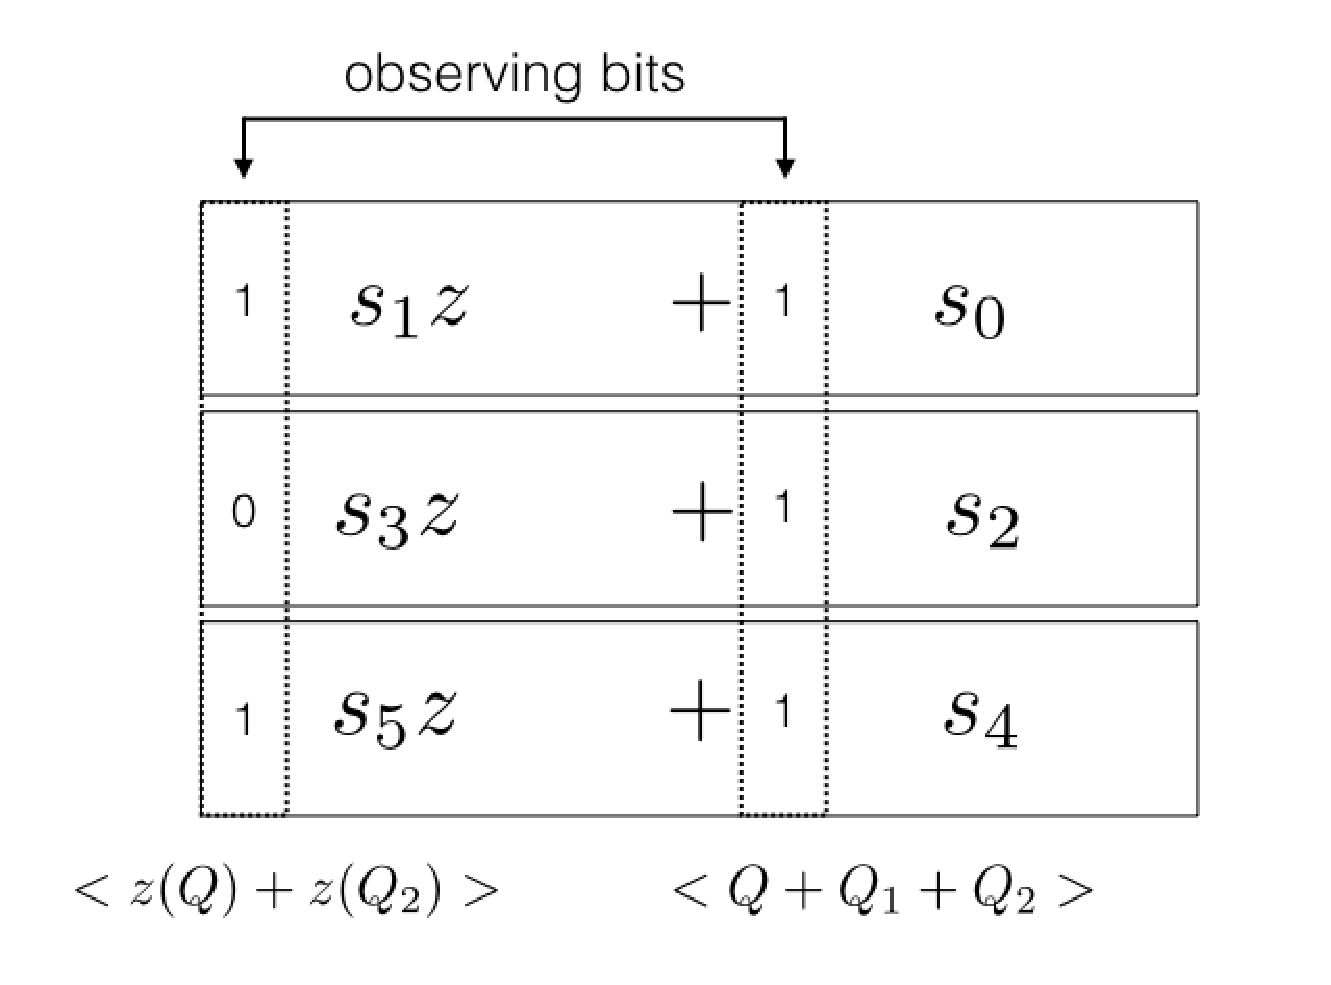
\includegraphics[width=.8\columnwidth]{z_sm.eps}
\caption{Multi-scalar multiplication of $s$ with Frobenius mapping.}
\label{fig:z_sml}
\end{figure}

As shown in Figure \ref{fig:z_sml}, during scalar multiplication, we are considering 3 pair of coefficients of $z$-adic representation as shown in  \eqref{eq:sclar_final_rep}. If we consider 6-coefficients for parallelization, it will require $2^6 \times 2$ pre-computed points. The chance of appearing each pre-computed point in the calculation will be only once that will cause redundancy.  

\subsubsection{Re-mapping rational points from $E'(\FQTH)$ to $E(\FQEN)$}
 After the multi-scalar multiplication, we need to remap the result to $\FQEN$. For example let us consider re-mapping of $Q' =(x',y') \in E'(\FQTH)$ to $Q =(Av\theta,Bv) \in E(\FQEN)$. From \eqref{thta2_4}, \eqref{thta_3} and \eqref{eq.sextic_div_theta} it can be obtained as follows:
 \begin{subequations}
 \begin{eqnarray}
 x i^{-1}\theta^{4} & = & Av\theta, \nonumber \\
 y i^{-1}\theta^{3} & = & Bv, \nonumber
 \end{eqnarray}
 \end{subequations}
  which resembles that $Q= (Av\theta, Bv)$. Therefore it means that multiplying $i^{-1}$ with the $Q'$ coordinates and placing the resulted coefficients in the corresponding position of the coefficients in $Q$, will map $Q'$ to $Q$.
This mapping costs one $\FQTH$ inversion of $i$ which can be pre-computed and one $\Fp$ multiplication.

\section{Simulation result evaluation}
This section shows experimental result with the calculation cost.
 In the experiment we have compared the proposed method with three well studied method of scalar multiplication named binary method, sliding-window method and non-adjacent form (NAF) method. 
The mother parameter $z$ is  selected according to the suggestion of Scott et al. \cite{kss_param} to obtain $p = 508 \approx 511$-bit and $r =  376 \approx 384$-bit  to simulate in 192-bit security level.
Table \ref{parameters} shows the parameter settings considered for the simulation.

\renewcommand{\baselinestretch}{1.5}
\begin{table}[htb]
	\begin{center}
		\caption{Parameter settings used in the experiment}
		%\resizebox{0.7\columnwidth}{!}{
		\begin{tabular}{|c|c|}
			\hline
			Defined KSS curve & $y^2 = x^3 + 11$ \\ \hline
			Mother parameter $z$ & 65-bit \\ \hline
			Characteristics  $p(z)$ & 511-bit \\ \hline
			Order  $r(z)$ & 376-bit \\ \hline
			Frobenius trace $t(z)$ & 255-bit \\ \hline
			Persuadable security level & 192-bit \\ \hline
		\end{tabular}
		%}
		\label{parameters}
	\end{center}
\end{table}
\renewcommand{\baselinestretch}{1.0}

Table \ref{tab1} shows the environment, used to experiment and evaluate the proposed method.  
\renewcommand{\baselinestretch}{1.5}
\begin{table}[!ht]
\renewcommand{\arraystretch}{1.3}
\centering
\caption{ Computational Environment}
\label{tab1}
\resizebox{\columnwidth}{!}{
\begin{tabular}{|c|c|c|}
\hline 
 & PC & iPhone6s \\ 
\hline \hline 
CPU {\textsuperscript{*}} & \quad 2.7 GHz Intel Core i5 \quad & \quad Apple A9 Dual-core 1.84 GHz \quad \\ 
\hline 
Memory & 16 GB & 2 GB \\ 
\hline 
OS & Mac OS X 10.11.6 &  iOS 10.0 \\ 
\hline 
Compiler & gcc 4.2.1 & gcc 4.2.1 \\ 
\hline 
\quad Programming Language \quad  & C & Objective-C, C \\ 
\hline 
Library &  GMP 6.1.0 & GMP 6.1.0\\ 
\hline 
\multicolumn{3}{l}{\textsuperscript{*}\footnotesize{Only single core is used from two cores.}}\\
\end{tabular} 
}
\end{table}
\renewcommand{\baselinestretch}{1.0}

In the experiment 100 random scalar numbers of size less than order $r$ ( 378-bit) is generated.
13  ECA counted for pre-computed rational points is taken into account while the average is calculated for the proposed method.
Window size of 4-bit is considered for sliding-window method. 
Therefore 14 pre-computed ECA is required. 
In addition, average execution time of the proposed method and the three other methods is also compared along with the operation count.

In what follows, ``\textit{\textbf{With isomorphic mapping}}'' refers that  skew Frobenius mapping technique is applied for Binary, Sliding-window and NAF methods. Therefore the scalar multiplication is calculated in $\FQTH$ extension field.
And for Proposed method it is skew Frobenius mapping with multi-scalar multiplication. 
On the other hand ``\textit{\textbf{Without isomorphic mapping}}'' denotes that Frobenius map is not applied for any of the methods.
In this case, all the scalar multiplication is calculated in $\FQEN$ extension field.

%\medskip\noindent
\renewcommand{\baselinestretch}{1.5}
\begin{table}[!ht]
\label{tab_operation}
\caption{Comparison of average number of ECA and ECD }
\resizebox{\columnwidth}{!}{
\begin{tabularx}{0.5\textwidth}{|c *{3}{|Y}|}
\cline{2-3}
\multicolumn{1}{c|}{} & 
\multicolumn{2}{c|}{Count of average number of ECA, ECD}\\
\hline
 Methods & \#ECA & \#ECD  \\
\hline
 Binary  & 186 & 375 \\
 \hline
 Sliding-window  & 102 & 376 \\
 \hline
 NAF &  127 & 377  \\
 \hline
 Proposed & 123 & 64 \\
\hline
\end{tabularx}
}
\end{table}
\renewcommand{\baselinestretch}{1.0}
In Table \ref{tab_operation} the operations of the \textit{Proposed} method are counted in $\FQTH$. On the other hand for Binary, Sliding-window and NAF method, the operations are counted in $\FQEN$.  The table clearly shows that in the \textit{Proposed} method requires about 6 times less ECD than any other methods.
The number of ECA is also reduced in the \textit{Proposed} method by about 30\% than binary method and almost same number of ECA of NAF. 

\renewcommand{\baselinestretch}{1.5}
\begin{table}[!ht]
\centering
\caption{Comparison of execution time in [ms] for scalar multiplication}
\label{tab_execution}
\resizebox{\columnwidth}{!}{
\begin{tabularx}{0.6\textwidth}{|c *{5}{|Y}|}
\cline{2-5}
\multicolumn{1}{c|}{} & 
\multicolumn{4}{c|}{Execution time in [ms] }\\
\cline{2-5}
\multicolumn{1}{c|}{} & 
 \multicolumn{2}{c|}{With isomorphic mapping}&
 \multicolumn{2}{c|}{Without isomorphic mapping }\\
\hline
 Methods & 
PC &  iPhone6s &
PC &  iPhone6s \\
\hline
 Binary  
 &  $5.4 \times 10^1$  &  $8.4 \times 10^1$ 
  &  $1.2 \times 10^3$  &  $1.8 \times 10^3$ \\
 \hline
 Sliding-window 
  &  $4.8 \times 10^1$  &  $7.5 \times 10^1$ 
  &  $1.0 \times 10^3$  &  $1.6 \times 10^3$ \\
 \hline
 NAF
  &  $5.3 \times 10^1$  &  $7.7 \times 10^1$ 
  &  $1.6 \times 10^3$  &  $1.7 \times 10^3$ \\
 \hline
 Proposed
  &  $1.6 \times 10^1$  &  $2.4 \times 10^1$ 
  &  -  &  - \\
\hline
 Multi-scalar  (only)
  &  -  &  -
  &  $3.4 \times 10^2$  &  $5.5 \times 10^2$ \\
\hline
\end{tabularx}
}
\end{table}
\renewcommand{\baselinestretch}{1.0}

Analyzing  Table \ref{tab_execution}, we can find that when isomorphic mapping  and skew Frobenius mapping is not adapted for  Binary, Sliding-window and NAF, then the scalar multiplication of  proposed method is more than 60 times faster than other methods. However when isomorphic mapping  is applied for the other methods then our proposed technique is more than 3 times faster. Another important comparison shows that when only multi-scalar multiplication is applied then our proposed methods is about 20 times faster. 
In every scenario our proposed method is faster than the other commonly used approaches.


The main focus of this experiment is to evaluate the  acceleration ratio of scalar multiplication by applying the proposed approach on $\g2$ rational point group of  KSS curve of embedding degree 18. The experiment does not focus on efficiently implementing scalar multiplication for certain environment. 

\section{Conclusion and future work}
In this paper we have proposed an efficient method to calculate elliptic curve scalar multiplication using skew Frobenius mapping  over KSS curve in context of pairing based cryptography. 
The simulation result shows that multi-scalar multiplication after applying skew Frobenius mapping in $\g2'$ can accelerate the scalar multiplication in $\g2 \subset E(\FQEN)$ by more than 60 times than scalar multiplication of $\g2$ rational point directly in $\FQEN$. 
In the previous work of Sakemi et al. \cite{sakemi_skew} has proposed skew Frobenius map for $\g1$ rational point defined over BN curve. 
As a future work we would like to apply such approach on $\g1$ rational point defined over KSS curve.
Together with the proposed method, the skew Frobenius mapping of $\g1$ will remarkably accelerate scalar multiplication over KSS curve in the context of pairing based cryptography. 
